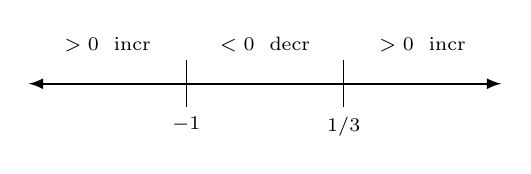
\begin{tikzpicture}[>=latex]

\draw [<->, thick] (-3,0) -- (3,0);
\foreach \x / \y  in %
					{%
					-1/{$-1$},%
					1/{1/3},%
					}
		{\draw (\x,-.3) node[below] {\scriptsize \parbox{40pt}{\centering \y}} -- (\x,.3);}
		
\draw (-2,.5) node {\scriptsize \parbox{50pt}{\centering $\fp>0$ \ incr }};
\draw (0,.5) node {\scriptsize \parbox{50pt}{\centering $\fp<0$ \ decr }};
\draw (2,.5) node {\scriptsize \parbox{50pt}{\centering $\fp>0$ \ incr }};
%\draw (3.75,.5) node {\scriptsize \parbox{50pt}{\centering $\fp>0$ \ incr \vskip 3pt $\fpp<0$ \ c. up}};


\end{tikzpicture}